\chapter{System Specification, Design, and Implementation}\label{ch:specs_design_implem}

This chapter details the proposed solution, in three sections.
Section~\ref{sec:specs} discusses the requirements and specifications.
Section~\ref{subsec:prop_vision} presents the system design.
Finally, Section~\ref{sec:impl} describes the system implementation.

\section{System Specification}\label{sec:specs}
The goal of this dissertation was to extract vision-based information relevant to a 5G network.
This information should be available in near real-time to relevant entities of the network architecture upon subscription.
This solution envisions obstacle-aware networks and should enable a RAN to autonomously control the BS' placement and configuration based on the environment perception provided by the vision-based information.

\subsection{System Requirements}\label{subsec:system-requirements}

The scenario is set in an indoor environment, where it is determined if common objects will impact the LOS between a gNB and a UE\@.
This concept is inspired in the anechoic chamber seen in Figure~\ref{fig:chamber_converge}.
In this dissertation, we will make use of a single UE and a mobile BS\@.
Figure~\ref{fig:my_chamber} presents the overall intended system.

\textcolor{red}{Figure to ilustrate system}
\begin{figure}[H]
    \centering
    
\includegraphics[width=0.7\linewidth]{figures/uporto-feup}
    \caption[Another figure]{Another figure}
    \label{fig:my_chamber}
\end{figure}

To achieve this, specific system requirements were established to ensure the efficient detection, tracking, and dissemination of obstacles information within the 5G network.

The detailed functional and non-functional requirements of the Computer Vision Module and its interface with the network are as follows:

\begin{enumerate}
    \item \textbf{Functional Requirements}
    \begin{enumerate}
        \item Detect and track objects in near real-time using computer vision algorithms.
        \item Identify specific obstacles and predict potential blockages.
        \item Send well-defined messages to a novel O-RAN xApp for further processing and decision-making.
        \item Ensure interoperability with the 5G network components via standardized messaging protocols. % should i use standarized, since there is no standard for it, i created a structure?
    \end{enumerate}
    \item \textbf{Non-Functional Requirements}
    \begin{enumerate}
        \item Maximize processing speed resorting to parallel processing on the GPU whenever possible\@.
        \item Minimize messaging latency ensuring rapid response by the xApp for optimal connection maintenance.
        \item High accuracy in object detection and tracking to minimize false positives and negatives.
        \item The solution should be scalable to handle multiple video streams, Base Stations, and UEs, allowing for broader deployment in various network environments.
        \item The system must use standardized messaging formats to ensure interoperability with different network components and vendors.
        \item The vision module and communications system should be robust, with mechanisms for error detection and recovery to maintain continuous operation.
        The model and its parameters are fundamental to ensure reliability. % how can i prove it?
    \end{enumerate}
\end{enumerate}

These requirements translate into Table ~\ref{tab:spec}, containing system specifications:

\begin{table}[H]
\caption{System specifications.}
\label{tab:spec}
\centering
\resizebox{\textwidth}{!}{%
\begin{tabular}{|l|p{12cm}|}
\hline
\textbf{Specification} & \textbf{Description} \\ \hline
\textbf{Detection and tracking} & Use YOLOv5 Ultralytics~\cite{Ultralytics_repo} and BoT-SORT~\cite{botsort} for high accuracy and optimized speed. \\ \hline
\textbf{Messaging} & Encode messages using ASN.1 definitions~\cite{ITU_ASN1}. \newline Transmit messages via Stream Control Transmission Protoco(SCTP). \newline Include relevant information such as object ID, type, position ( cartesian coordinates), and confidence score. \\ \hline
\end{tabular}}
\end{table}

These specifications ensure that the Vision Module meets the requirements necessary for integration and operation within a 5G network environment.


Following these requirements and specifications, the system architecture was designed to facilitate efficient data processing.

\section{System Design}\label{sec:design}

\begin{figure}[H]
    \centering
    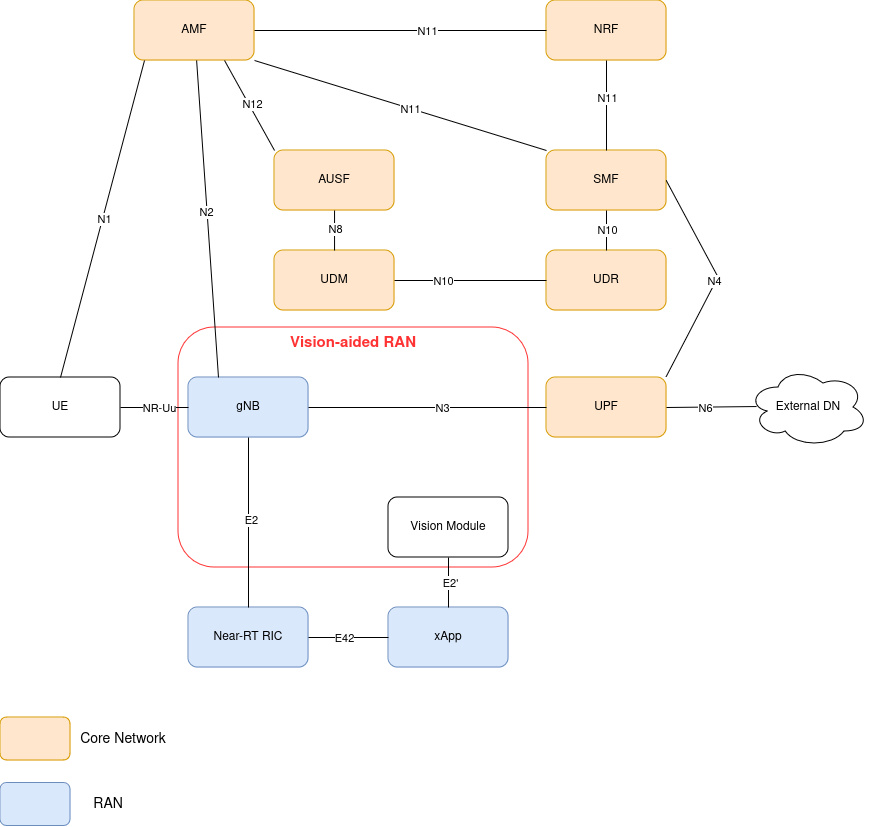
\includegraphics[width=0.7\linewidth]{figures/Syst_Arch.drawio}
    \caption[System architecture of the proposed solution]{System architecture of the proposed solution}
    \label{fig:my_arch}
\end{figure}

% draw: SMF[x], SPGWU[x], AMF[x], AUSF, UDM, UDR, mysql, NRF ext DN[x]
% requires improvements

\textcolor{red}{Confirm acronism}
The proposed architecture, shown in Figure~\ref{fig:my_arch}, includes a UE requiring 5G connectivity.
The 5G connection process begins with the UE initiating a connection request to the gNB, which then forwards the request to the AMF\@.
The gNB acts as the intermediary between the UE and the 5G core network, managing the radio resources, handling data transmission, and ensuring seamless connectivity as the UE moves.
The AMF authenticates the UE using credentials stored in the UDM. Upon successful authentication, the UE is granted  network access.
Subsequently, the AMF and UPF establish a data session for the UE, configuring the necessary resources for data transmission.
User data is transmitted between the UE and the UPF via the gNB\@.
The UPF routes the data to and from external networks, ensuring data forwarding.

%------------ move to another place
%The 5G Core Network is responsible for managing the overall network functions, including authentication, mobility management, and routing of data.
%In our solution, both the RAN and the core are deployed within the same processing unit to maintain efficiency, mobility and simplicity.
%The AMF is a critical component of the 5G core that handles user authentication and mobility management.
%When a UE attempts to connect to the network, the AMF verifies the user's credentials and manages their session as they move across different cells in the network.

%The User Plane Function (UPF) manages the user data traffic, ensuring that data packets are efficiently routed between the UE and external data networks.
%It plays a pivotal role in delivering low-latency, high-bandwidth services to the end-users.
%Another essential core network function is the Unified Data Management (UDM), responsible for handling subscriber data and profiles.
%It ensures that user data is consistent and accessible across the network, supporting seamless user experiences.
%The User Plane Function (UPF) manages the user data traffic, ensuring that data packets are efficiently routed between the UE and external data networks.
%It plays a pivotal role in delivering low-latency, high-bandwidth services to the end-users.
%Another essential core network function is the Unified Data Management (UDM), responsible for handling subscriber data and profiles.
%It ensures that user data is consistent and accessible across the network, supporting seamless user experiences.

%To ensure the mobility and efficiency of our solution, the RAN and the core network components are deployed within the same processing unit.
%This integration offers several advantages.
%By colocating the RAN and core network functions, data processing and transmission delays are minimized, resulting in a more responsive network.
%The mobile RAN can seamlessly maintain connectivity with the UE, even when the gNB is moving, without relying on distant core network infrastructure.
%Having the RAN and core in a single unit simplifies the deployment process, making it easier to set up and manage the network in various locations, whether stationary or on the move.
%-------------------

In our solution, the RAN can be repositioned based on environment conditions that may affect the RF signal propagation\@.
These conditions, perceived and reported by the Vision Module (VM).
This enables, as well as RF metrics such as SNR, allow the RAN to manage its placement.
In order to integrate of Computer Vision into the 5G architecture, we took advantage of the Near-RT RIC, specified by O-RAN, to deploy a xApp responsible for handling both RF metrics and the VM messages.
Communications between the VM and the xApp, is achieved through interface E2', based on the O-RAN E2 interface and E2 Application Protocol (E2AP).
E2' interface supports reliable data exchange using a SCTP socket connection (cf.
Figure~\ref{fig:stack}) along with an ASN.1 definition to structure the messages.
The use of ASN.1 ensures that the standarized message formats , promoting interoperability and efficiency in data exchange.
This design enables the VM to communicate with the xApp, allowing the integration of data extracted from video for the mobile RAN management.

\begin{figure}[H]
    \centering
    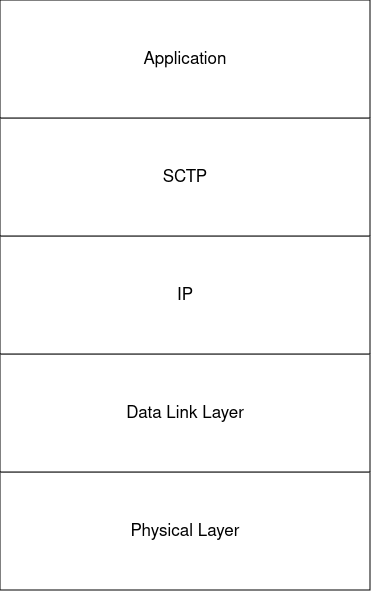
\includegraphics[width=0.2\linewidth]{figures/VisionModule_ProtocolStack.drawio(2)}
    \caption[Proposed Vision Module Protocol Stack]{Proposed vision module protocol stack.}
    \label{fig:stack}
\end{figure}


\subsection{Proposed Vision Module}\label{subsec:prop_vision}
The proposed Vision Module uses Computer Vision techniques to extract information about obstacles within the video camera's field of view.
This system processes video frames to detect and track obstacles, while sending messages with relevant information to services connected.
The module sends five types of messages: blockage, prior to blockage, post blockage, the location of the UE and frame processed.
Table~\ref{tab:message_type} summarizes each message type.
Each message is explained further in the following sections.

\begin{table}[H]
    \caption{Summary of each message type.}
    \label{tab:message_type}
    \centering
    \resizebox{\textwidth}{!}{%
        \begin{tabular}{|l|p{12cm}|}
            \hline
            \textbf{Type of message} & \textbf{Description} \\ \hline
            Blockage Messages & Sent when an obstacle is currently blocking the UE. \\ \hline
            Prior Blockage Messages & Sent when an obstacle is predicted to block the UE based on its current trajectory. \\ \hline
            Post Blockage Messages & Sent when an obstacle that was previously blocking the UE is no longer doing so. \\ \hline
            UE Location Messages & Provide the current location of the UE. \\ \hline
            Frame Processed & Provide information that a frame of the video was processed. \\ \hline
        \end{tabular}}
\end{table}

VM includes functionalities responsible for information exchange, detection and tracking, image processing, and auxiliary functions, such as coordinates transformations and definition of the structure of the messages.
We present a high level overview of the developed VM\@.

The video processing starts capturing frames from the video camera.
One frame is processed at a time.
The UE has an ArUco marker in order to identify its placement.
ArUco markers are square markers commonly used in CV applications to simplify the process of camera pose estimation and object tracking.
They are easily detectable in images and videos, providing a reliable method for identifying and localizing objects in various environments.
In order to simply the differentiation between UE and obstacles, they were chosen to represent the position of the UE\@.

OpenCV is responsible for identifying ArUco marker and returning the ROI corresponding to the marker, as well as its identification.
Periodically, the VM sends a message containing the location (in normalized Cartesian coordinates) of the UE within the frame\@.
Following this, \emph{yolov8n}, a YOLO pre-trained model jointly with BoT-SORT, is responsible for detecting and tracking the obstacles in the frame.
To improve control over frame selection for tracking detected objects, we have set specific parameters that allow timing adjustments in object detection, extending the Ultralytics API and enabling us to adjust the duration an obstacle remains detectable in the frame.
Adjusting the persistence time is important because it allows for more accurate and stable tracking of objects, especially in dynamic environments.
By fine-tuning how long an obstacle remains detectable in the frame, we can prevent sudden disappearances and reappearances of objects, leading to smoother and more reliable tracking.
This enhances the overall performance of object detection systems and is particularly useful in applications where consistent monitoring is critical.

The main returned value by Ultralytics is a track history containing a unique identifier of the obstacle and its associated last positions (in normalized Cartesian coordinates), alongside its classes and confidence scores.
If it is noticed that there is a difference between the last visible ArUco marker and the current seen ones, the module checks if the obstacle last position intercepts the ArUcos position.
If an intersection is confirmed, the module generates a Blockage message, indicating that an obstacle blocked the UE\@.
Once the UE is unblocked, the module issues a Post Blockage message, indicating the reestablishment of the LoS between gNB and UE.

Additionally, the module is capable of predicting with some anticipation that an obstacle seen by the video camera will block the UE\@.
This is done using the tracking history constructed from the tracking results.
This enables the calculation of the objects' velocity.
We can then estimate the future positions and calculate whether the projected bounding boxes will intercept the ArUco.
This prediction allows us to reposition the gNB to maintain of the LoS and the channel quality, assessed by the SNR\@.

The messages consist of a header and a payload.
The header of all messages is presented in Table~\ref{tab:header}.


\begin{table}[H]
    \caption{Components of each message header.}
    \label{tab:header}
    \centering
    \resizebox{\textwidth}{!}{
        \begin{tabular}{|c|c|}
            \hline
            \textbf{Field} & \textbf{Description} \\ \hline
            messageType & Identifies the type of the message. \\ \hline
            timestamp & Identifies the  timestamp when the message was created. \\ \hline
            sourceId & Identifies the source of the message.
            In this case, the Vision Module.\\ \hline
            destinationId & Identifies the intended recipient of the message.
            In this case, the xApp. \\ \hline
        \end{tabular}
    }
\end{table}

The payload varies by message type.
Each message requires different processing to extract the required information, as mentioned previously.
The following subsections further present each message type.

\subsection{Prior to Blockage Messages}\label{subsec:prediction-of-blockage-messages}

To infer that an obstacle will block the LoS between the gNB and the UE, it is necessary to obtain the obstacles' tracking history.
We achieve this by storing data over several frames, using the YOLO and BoT-SORT algorithms.
Once the tracking history is established, we modeled the object's movement assuming a constant velocity.
This has proven effective for handling typical indoor movements, such as people walking or objects being moved.
By calculating the object's velocity, it is possible to predict its future positions in upcoming video frames.
This allows us to determine whether the obstacle will interrupt the LoS\@.
If the module predicts an impending blockage, it generates a message containing the information summarized in Table~\ref{tab:future_block_message}.


\begin{table}[H]
    \caption{Components of the Prior to Blockage message's payload}
    \label{tab:future_block_message}
    \centering
    \resizebox{\textwidth}{!}{
        \begin{tabular}{|c|c|}
            \hline
            \textbf{Field} & \textbf{Description} \\ \hline
            obstacleID & Unique identifier for the obstacle, provided by the tracking. \\ \hline
            obstacleType & Type of obstacle detected. \\ \hline
            obstacleLocation & Location of the detected obstacle within the frame (normalized Cartesian coordinates). \\ \hline
            obstacleVelocity & Velocity of the detected obstacle (normalized vector). \\ \hline
            obstacleConfidence & Confidence level in the identification of the object. \\ \hline
            timeToCross & Predicted time the obstacle will obstruct the UE. \\ \hline
            ueId & Identifier for the UE; in this case, its ArUco identifier. \\ \hline
        \end{tabular}
    }
\end{table}




\subsection{Blockage messages}\label{subsec:blocking-messages}
To detect if an obstacle is blocking the LoS between the gNB and the UE, the system must verify whether the obstacle’s current position corresponds to its last known position where the ArUco marker was detected.
This involves comparing the obstacle's most recent recorded position with the last seen coordinates of the UE\@.
If these positions overlap, the system generates a blockage alert.
Table~\ref{tab:block_payload} presents the payload fields of this message.


\begin{table}[H]
    \caption{Components of the Blockage payload.}
    \label{tab:block_payload}
    \centering
    \resizebox{\textwidth}{!}{
        \begin{tabular}{|c|c|}
            \hline
            \textbf{Field} & \textbf{Description} \\ \hline
            obstacleID & Unique identifier for the obstacle, provided by the tracking. \\ \hline
            obstacleType & Type of obstacle detected. \\ \hline
            obstacleLocation & Location of the detected obstacle within the frame (normalized Cartesian coordinates). \\ \hline
            obstacleConfidence & Confidence level in the identification of the object. \\ \hline
            timeBlocked & Time the obstacle has been blocking, up to 5000 milliseconds (optional). \\ \hline
            ueId & Identifier for the UE, in this case its ArUco identifier. \\ \hline
        \end{tabular}
    }
\end{table}

The time limit for an object being considered \("\)blocked\("\) is set to 5 seconds, which matches the persistence time.
If  the object's blocking time exceeds this limit, the object will no longer be registered in the tracking model, ensuring that the object blocking the ArUco marker is no longer tracked.
This design choice ensures that the VM remains resilient when the UE is no longer in the frame or in LoS, even in situations without obstruction.


\subsection{Post Blockage}\label{subsec:past-blockage}
This message is sent to inform that the UE is no longer blocked by the obstacle.
When the system detects a blockage, it updates a list containing the state for each tracked object.
If the state changes from blocking to non-blocking, it triggers a past blockage message.
Table~\ref{tab:past_block_payload} presents the payload fields of this message.


\begin{table}[H]
    \caption{Components of the payload of Post Blockage message.}
    \label{tab:past_block_payload}
    \centering
    \resizebox{\textwidth}{!}{
        \begin{tabular}{|c|c|}
            \hline
            \textbf{Field} & \textbf{Description} \\ \hline
            obstacleID & Unique identifier for the obstacle, provided by the tracking. \\ \hline
            obstacleType & Type of obstacle detected. \\ \hline
            obstacleLocation & Location of the detected obstacle  within the frame (normalized Cartesian coordinates). \\ \hline
            obstacleConfidence & Confidence level in the identification of the object. \\ \hline
            ueId & Identifier for the UE; in this case, its ArUco identifier. \\ \hline
        \end{tabular}
    }
\end{table}


\subsection{Location of UEs}\label{subsec:location-of-ues}
The message presents the location data of the UEs, and Table~\ref{tab:ue_payload} presents the message payload.
To extract this information, detecting the bounding boxes of the markers associated with the UEs is necessary.
The system continuously monitors the movement of the UEs and transmits updates whenever changes are detected.
This process involves identifying and tracking the bounding boxes of the ArUco markers associated with the UEs and comparing the current visible ArUco IDs with the previously detected IDs.
This is done through buffering, temporarily storing changes to ensure accuracy and consistency.
Location reports are sent periodically when changes in the UEs' positions are confirmed.
This approach ensures precise and timely updates on the UEs' locations.

\begin{table}[H]
    \caption{Components of the UE Location message payload.}
    \label{tab:ue_payload}
    \centering
    \resizebox{0.7\textwidth}{!}{
        \begin{tabular}{|c|c|}
            \hline
            \textbf{Field} & \textbf{Description} \\ \hline
            ueLocation & Contains the location of the UE. \\ \hline
            ueId & Identifier for the UE, based on the ArUco ID. \\ \hline
        \end{tabular}
    }
\end{table}




\subsection{Frame Processed}\label{subsec:frame-processed}
In our system, frame processed messages play an important role in maintaining communications and monitoring the performance of the VM.
These messages are primarily designed to inform the xApp that the VM is actively running and processing frames.
Additionally, they allow tracking of the time taken to process each frame, which is essential for performance optimization and debugging purposes.

The frame processed message contains the following fields, as detailed in Table~\ref{tab:frame_proc_pay}:

\begin{table}[H]
    \caption{Components of the Frame Processed message payload.}
    \label{tab:frame_proc_pay}
    \centering
    \resizebox{0.7\textwidth}{!}{
        \begin{tabular}{|c|c|}
            \hline
            \textbf{Field} & \textbf{Description} \\ \hline
            frameID & Sequential identification number of the frame. \\ \hline
            timeProcessed & Time taken to process the frame in milliseconds. \\ \hline
        \end{tabular}
    }
\end{table}

These messages serve as heartbeat signals to the xApp, confirming the VM's operational status and performance.
By continuously sending frame processed messages, the system ensures that the xApp is kept up-to-date with the VM's activity.


\section{System Implementation}\label{sec:system-implementation}

This section presents the system designed to implement and evaluate the proposed solution.
The system, depicted in Figure~\ref{fig:design_arch}, is composed of two main logical units.
The first unit implements the 5G Core Network, the Near-RT RIC, and the Vision-aided gNB, while the second unit implements the UE\@.

\begin{figure}[H]
    \centering
    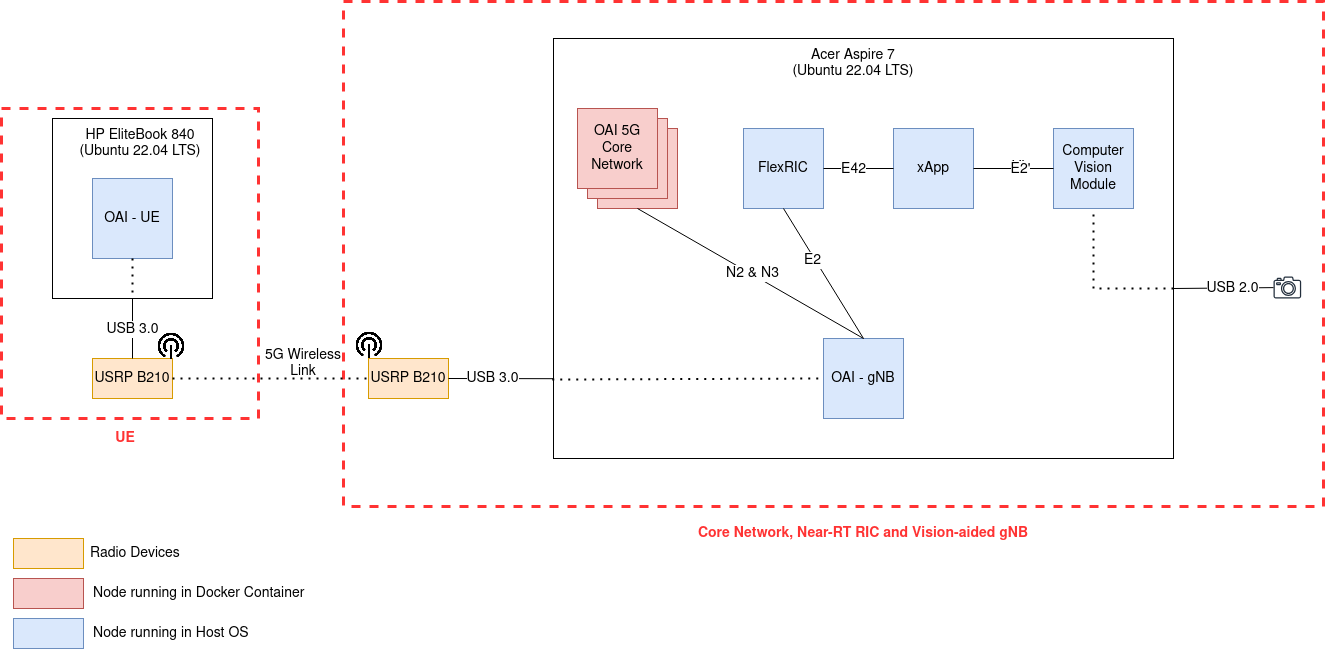
\includegraphics[width=0.75\linewidth]{figures/System Arch.drawio(3)}
    \caption[System architecture designed for implementing and evaluating the proposed solution]{System architecture designed for implementing and evaluating the proposed solution.}
    \label{fig:design_arch}
\end{figure}

The following subsections detail the hardware used in the implementation and the software packages choices.


\subsection{Software}\label{subsec:software}
This section presents the main software packages used to develop the Vision Module and implement the 5G network.
Beyond this, in the repository containing the VM~\ref{repository}, includes a file for reproducing the Python virtual environment.

\subsubsection{OpenCV}
There are several open-source software packages available for Computer Vision in Python.
Open Source Computer Vision Library (OpenCV)~\cite{opencv} is one of them.
OpenCV offers optimized algorithms for tasks such as object detection, image processing, and real-time video analysis.
Its well-documented API and cross-platform compatibility make it suitable for diverse applications.
OpenCV's large, active community provides extensive resources and support.
Additionally, OpenCV is the only library that directly supports ArUco Markers, which are essential for Augmented Reality applications involving the detection and tracking of unique binary-encoded markers for accurate localization and tracking.

Unlike scikit-image~\cite{Scikit-learn}, which excels in image processing tasks with functions for filtering, morphology, and segmentation, OpenCV offers a broader range of over 2500 optimized algorithms spanning image and video processing, object detection, and video camera calibration.
In contrast to Pillow (PIL Fork)~\cite{pillow}, which specializes in image format handling and basic manipulation, OpenCV provides tools for both basic and advanced computer vision applications.
Moreover, while SimpleCV~\cite{simplecv} simplifies OpenCV usage with a user-friendly interface, OpenCV's C++ backend and GPU acceleration capabilities enable superior performance, crucial for real-time processing and large-scale data operations.

In our proposed solution, OpenCV is used to:
\begin{itemize}
    \item \textbf{Obtain Frames:} OpenCV captures video frames from the video camera.
    It provides easy-to-use interfaces to capture and manipulate video streams from various input sources.
    \item \textbf{Detect ArUco Markers:} OpenCV includes modules for detecting ArUco markers, which are widely used in computer vision applications for video camera calibration, pose estimation, and augmented reality.
    In our solution, these markers help in identifying the UEs without needing to train the YOLO model to perceive such objects.
\end{itemize}

\subsubsection{Ultralytics YOLO}
As discussed in Section ~\ref{sec:CV}, Ultralytics YOLO (You Only Look Once)~\cite{ultralytics_docs} is a state-of-the-art, real-time object detection solution.
It is known for its speed and accuracy, making it suitable for applications requiring fast and reliable object detection and tracking.
While there are other solutions, also presented in Section~\ref{sec:CV}, we chose Ultralytics YOLO for its simplicity, and because it is suitable for the intended application and state-of-the-art object detection and tracking situations.

In our proposed solution, Ultralytics YOLO is employed to:
\begin{itemize}
    \item \textbf{Detection:} YOLO detects various objects in the frames captured by the video camera.
    Its real-time capabilities allow for the immediate identification of obstacles within the field of view.
    \item \textbf{Tracking:} YOLO’s tracking module is used to keep track of detected objects over successive frames.
    This is crucial for maintaining the continuity of object identification and predicting future positions of the obstacles. %BOTSORT and BYTETRACK
\end{itemize}

The combination of OpenCV and Ultralytics YOLO allows for robust detection, tracking, and message exchange functionalities in our vision module.
OpenCV handles the initial capture and processing of video frames, while YOLO and BoT-SORT perform the real-time detection and tracking of objects.
This integrated approach ensures that the vision module can effectively monitor and report obstacles, providing key information to subscriber services.

\subsubsection{ASN1Tools and ASN1C}
There are a few open-source libraries available for handling ASN.1.
ASN.1 provides a standardized way to define data structures that can be serialized and deserialized across different systems, ensuring interoperability and efficient data exchange.
Moreover, the E2 interface uses ASN.1 for encoding and decoding messages.
FlexRIC utilizes \emph{asn1c}~\cite{asn1c}; as such for simplicity, we chose the same for the xApp (client).
\emph{asn1c} is an open-source ASN.1 compiler that generates C/C++ code for ASN.1 data structures, supporting different encoding rules.
While this library also supports Python, we chose not to use it since there are simpler APIs specially tailored for Python development.
As for the Vision Module (Python server), we chose ASN1Tools because this solution offers certain advantages.

ASN1Tools~\cite{asn1tools} is a Python library that provides a simple way to handle ASN.1 data structures, through a straightforward API\@.
The library supports a range of ASN.1 specifications and encoding rules, including Basic Encoding Rules(BER), Distinguished Encoding Rules (DER), and Packed Encoding Rules(PER)\@.
Moreover, ASN1Tools is actively maintained, with regular updates and improvements.
This guarantees that we have access to the latest features and bug fixes, enhancing the reliability and stability of our system.
ASN1Tools is optimized for performance, allowing for fast encoding and decoding operations.
This optimization suits real-time applications like our Vision Module, where processing speed is essential to maintain system responsiveness and accuracy.

While other libraries such as pyasn1~\cite{pyasn1} and libtasn1~\cite{libtasn1} are available, they have certain limitations.
\emph{pyasn1}, for instance, is less efficient in terms of performance and has a more complex API\@.
libtasn1, part of the GNU project, is less user-friendly and not optimized for performance.


\subsubsection{5G Core Network, 5G gNB, and 5G UE}
The main open-source 5G software packages for implementing an O-RAN based architecture are OAI~\cite{openairinterface} and srsRAN~\cite{srslte}.
For our system, we chose OAI because it provides all the necessary components to deploy a 5G standalone network, including both the RAN and Core network.
In contrast, srsRAN only supports the deployment of the RAN, requiring an additional software package, such as OAI, to implement the Core network.

\subsubsection{Near-RT RIC}
The main open-source software packages able to implement a Near-RT RIC are Mosaic5G’s FlexRIC~\cite{flexric} and the O-RAN Software Community’s Near-RT RIC~\cite{oran-sc}.
FlexRIC was chosen for our solution due to its lightweight nature, launched from an executable file.

In contrast, the O-RAN RIC presents disadvantages in terms of its complexity and resource requirements.
It often demands more substantial computational resources and a more involved setup process, which are significant drawbacks for our solution.

\subsection{Hardware}\label{subsec:hardware}


\subsubsection{Core Network, FlexRIC, Computer Vision module and gNB}
The OAI Core Network, FlexRIC, the Vision Module, and the gNB were deployed on a laptop, the Acer Aspire A715-74G, which id shown in Figure~\ref{fig:computer_acer}.
The OAI Core was deployed using Docker containers, requiring a 4-core CPU, 16 GB of RAM and a minimum of 1.5 GB free storage for the Docker images.
FlexRIC does not have listed hardware requirements; however, during deployment, it was noticed that it is not resource-intensive, sufficing with the same requirements as the Core Network.
The xApp was deployed alongside FlexRIC to ensure reduced latency between the two components.
Also,  the implementation of interface E42 requires them to be run on the same computing unit.
For the gNB, the recommended hardware is 8 physical CPU cores and 32 GB of RAM\@.
Although the laptop used did not meet these requirements, it proved sufficient to run the OAI gNB software, as noted previously in~\cite{queiros2023autonomous}.

\begin{figure}[H]
    \centering
    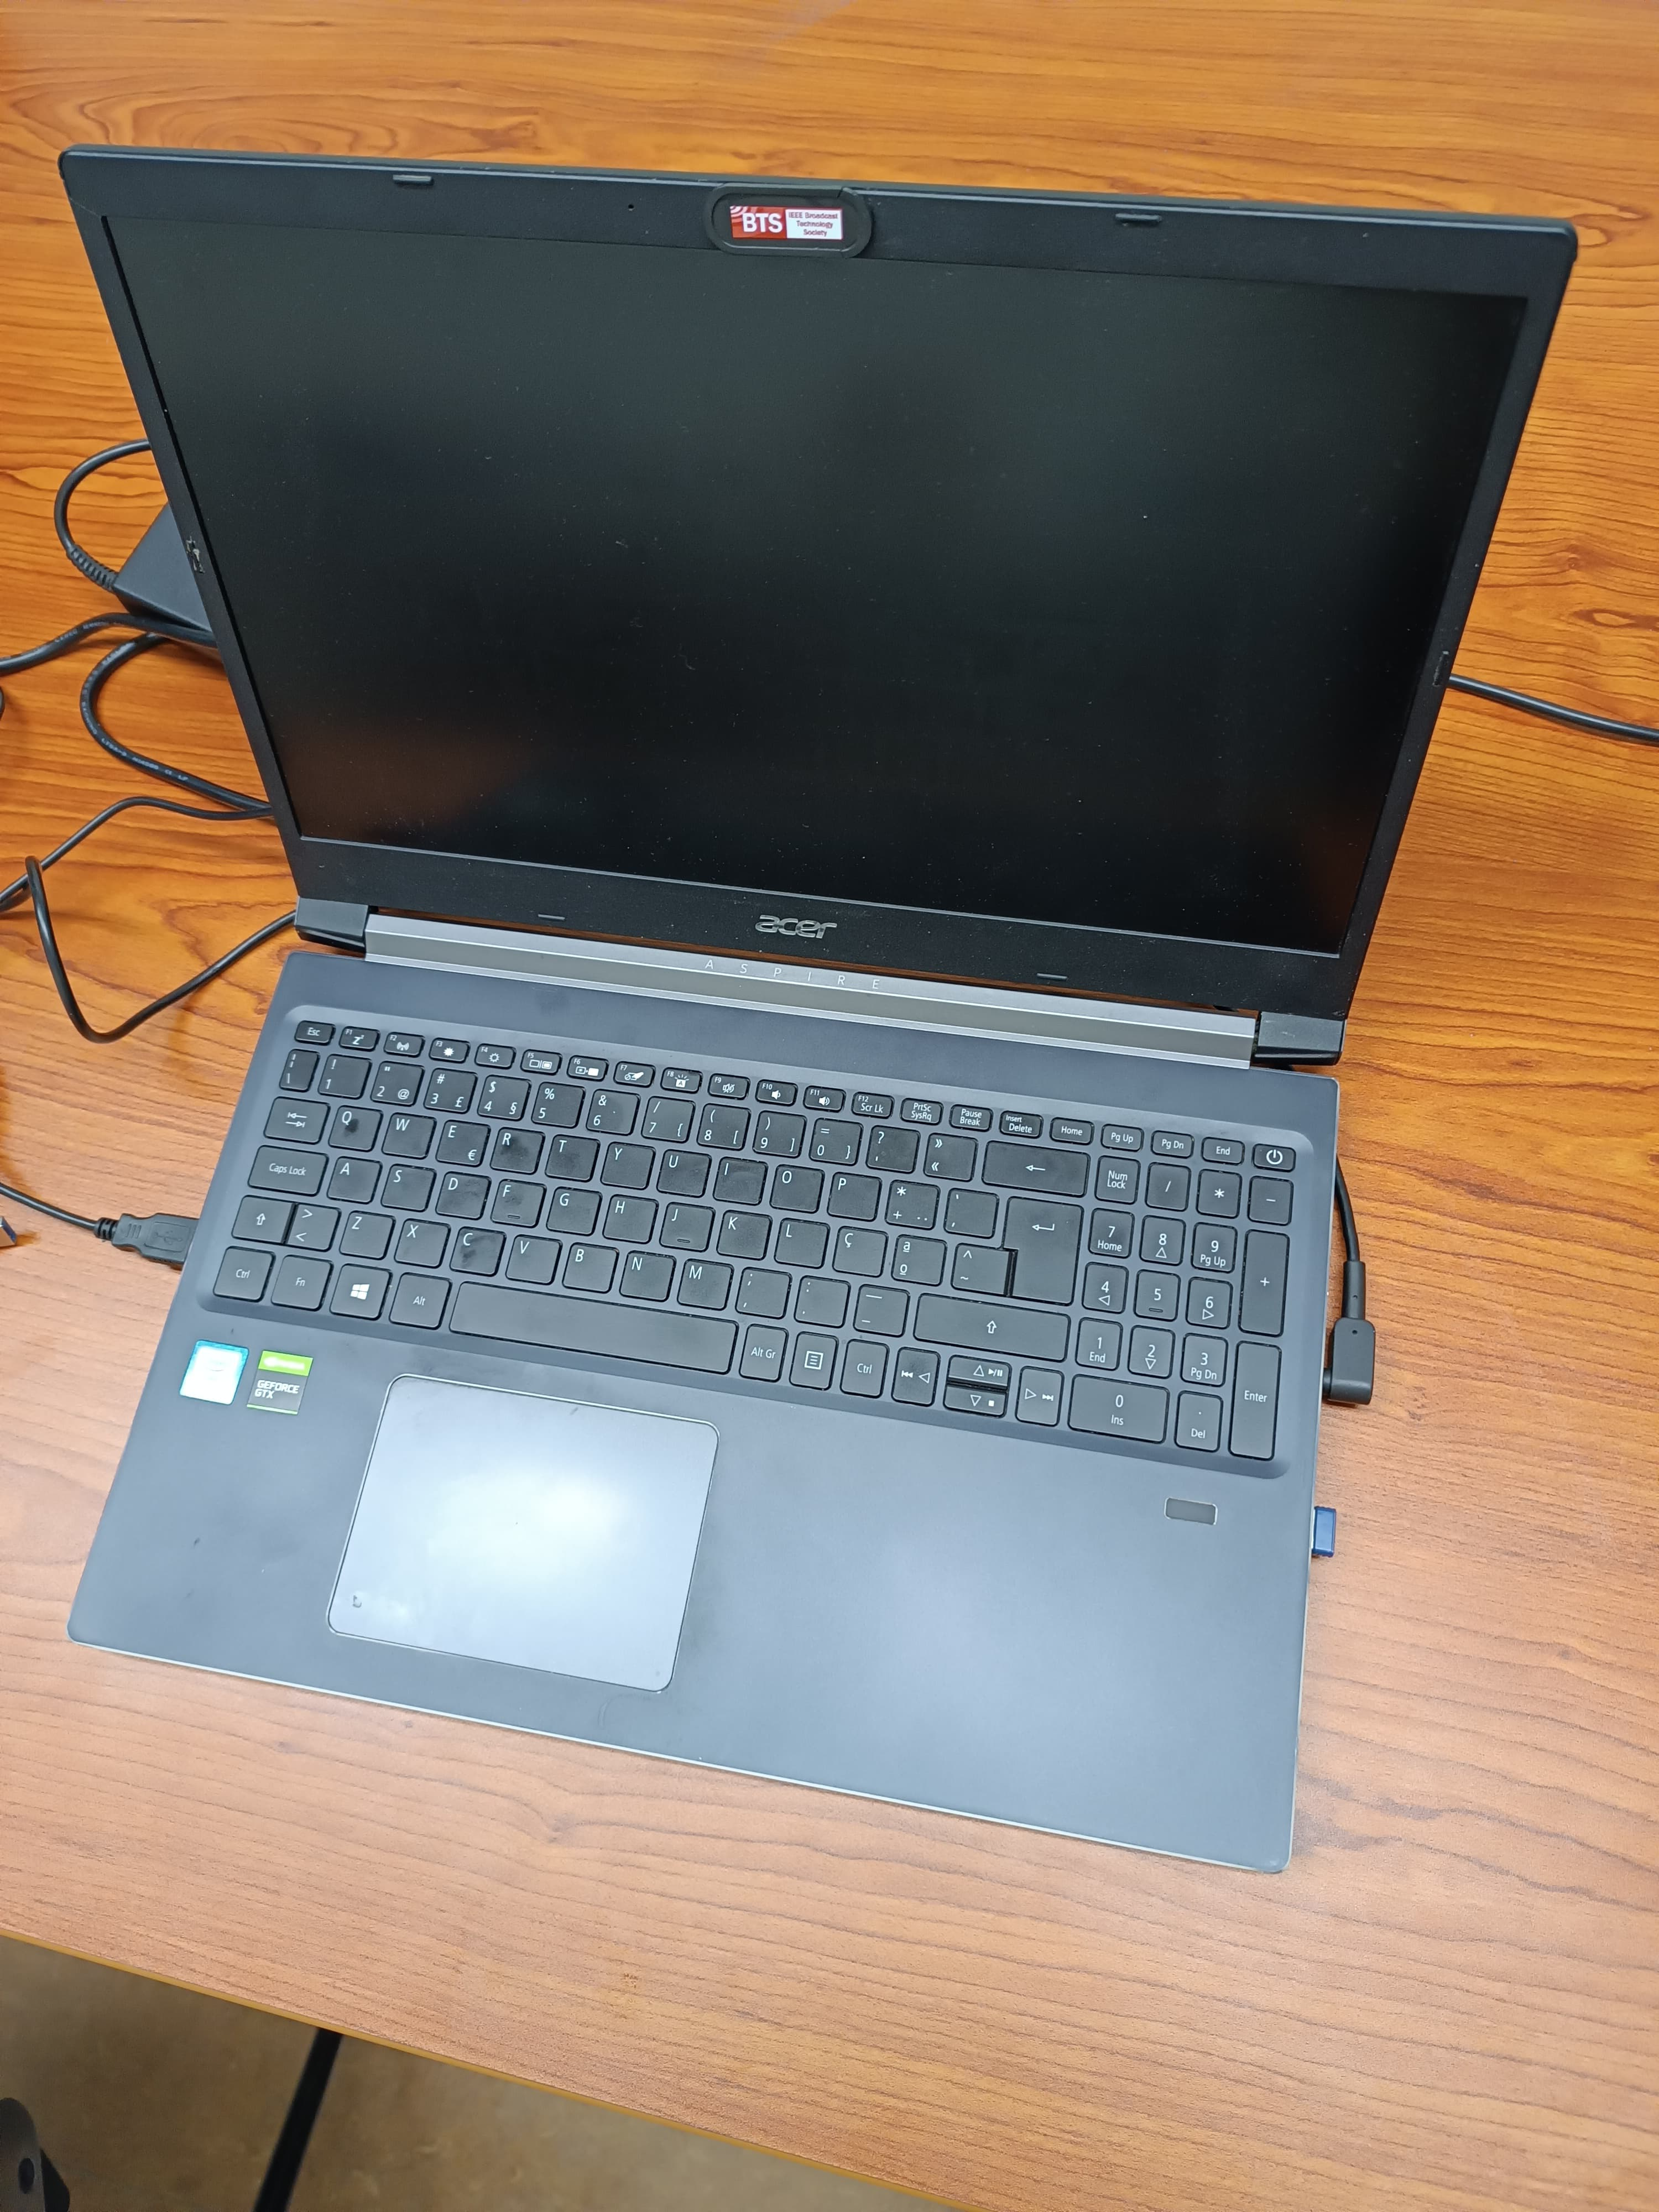
\includegraphics[width=0.3\linewidth]{figures/acer}
    \caption{Acer Aspire A715-74G Laptop}
    \label{fig:computer_acer}
\end{figure}

As for the Vision Module, the minimal hardware requirement is a CUDA-compatible GPU ~\cite{ultralytics_faq} for Ultralytics YOLO model to run properly.
Since a pre-trained model has proven sufficient to accurately detect and track objects for our solution, we did not require a high GPU capacity to train a model.

Table ~\ref{tab:specs_pc} presents the specification of the computer used.

\begin{table}[H]
    \caption{Specifications of the Acer Aspire A715-74G.}
    \label{tab:specs_pc}
    \begin{tabular}{|c|c|}
        \hline
        \textbf{Specification} & \textbf{Details} \\ \hline
        Processor                      &           Intel(R) Core(TM) i5-9300H CPU @ 2.40GHz   \\ \hline
        RAM                      &          16GB        \\ \hline
        Disk                      &   2 SSDs  (512GB and 256GB)         \\ \hline
        GPU                     &   GeForce GTX 1050 (3GB)      \\ \hline
        Operating System & Ubuntu 22.04.4 LTS                  \\ \hline
    \end{tabular}
\end{table}

For the Vision Module, we opted to use a webcam due to its simplicity and ease of integration.
The chosen model was LL-4196, offering Full HD (1920 x 1080 Pixels) resolution and supporting a frame rate of 30 frames/s\@.
This ensures that the video feed acquired is of high quality, providing sufficient detail and smooth motion, necessary for accurate computer vision processing.
The video camera connects to the computer using a USB 2.0 interface.
Figure~\ref{fig:camera} shows the video camera and its USB interface.

\begin{figure}[H]
    \centering
    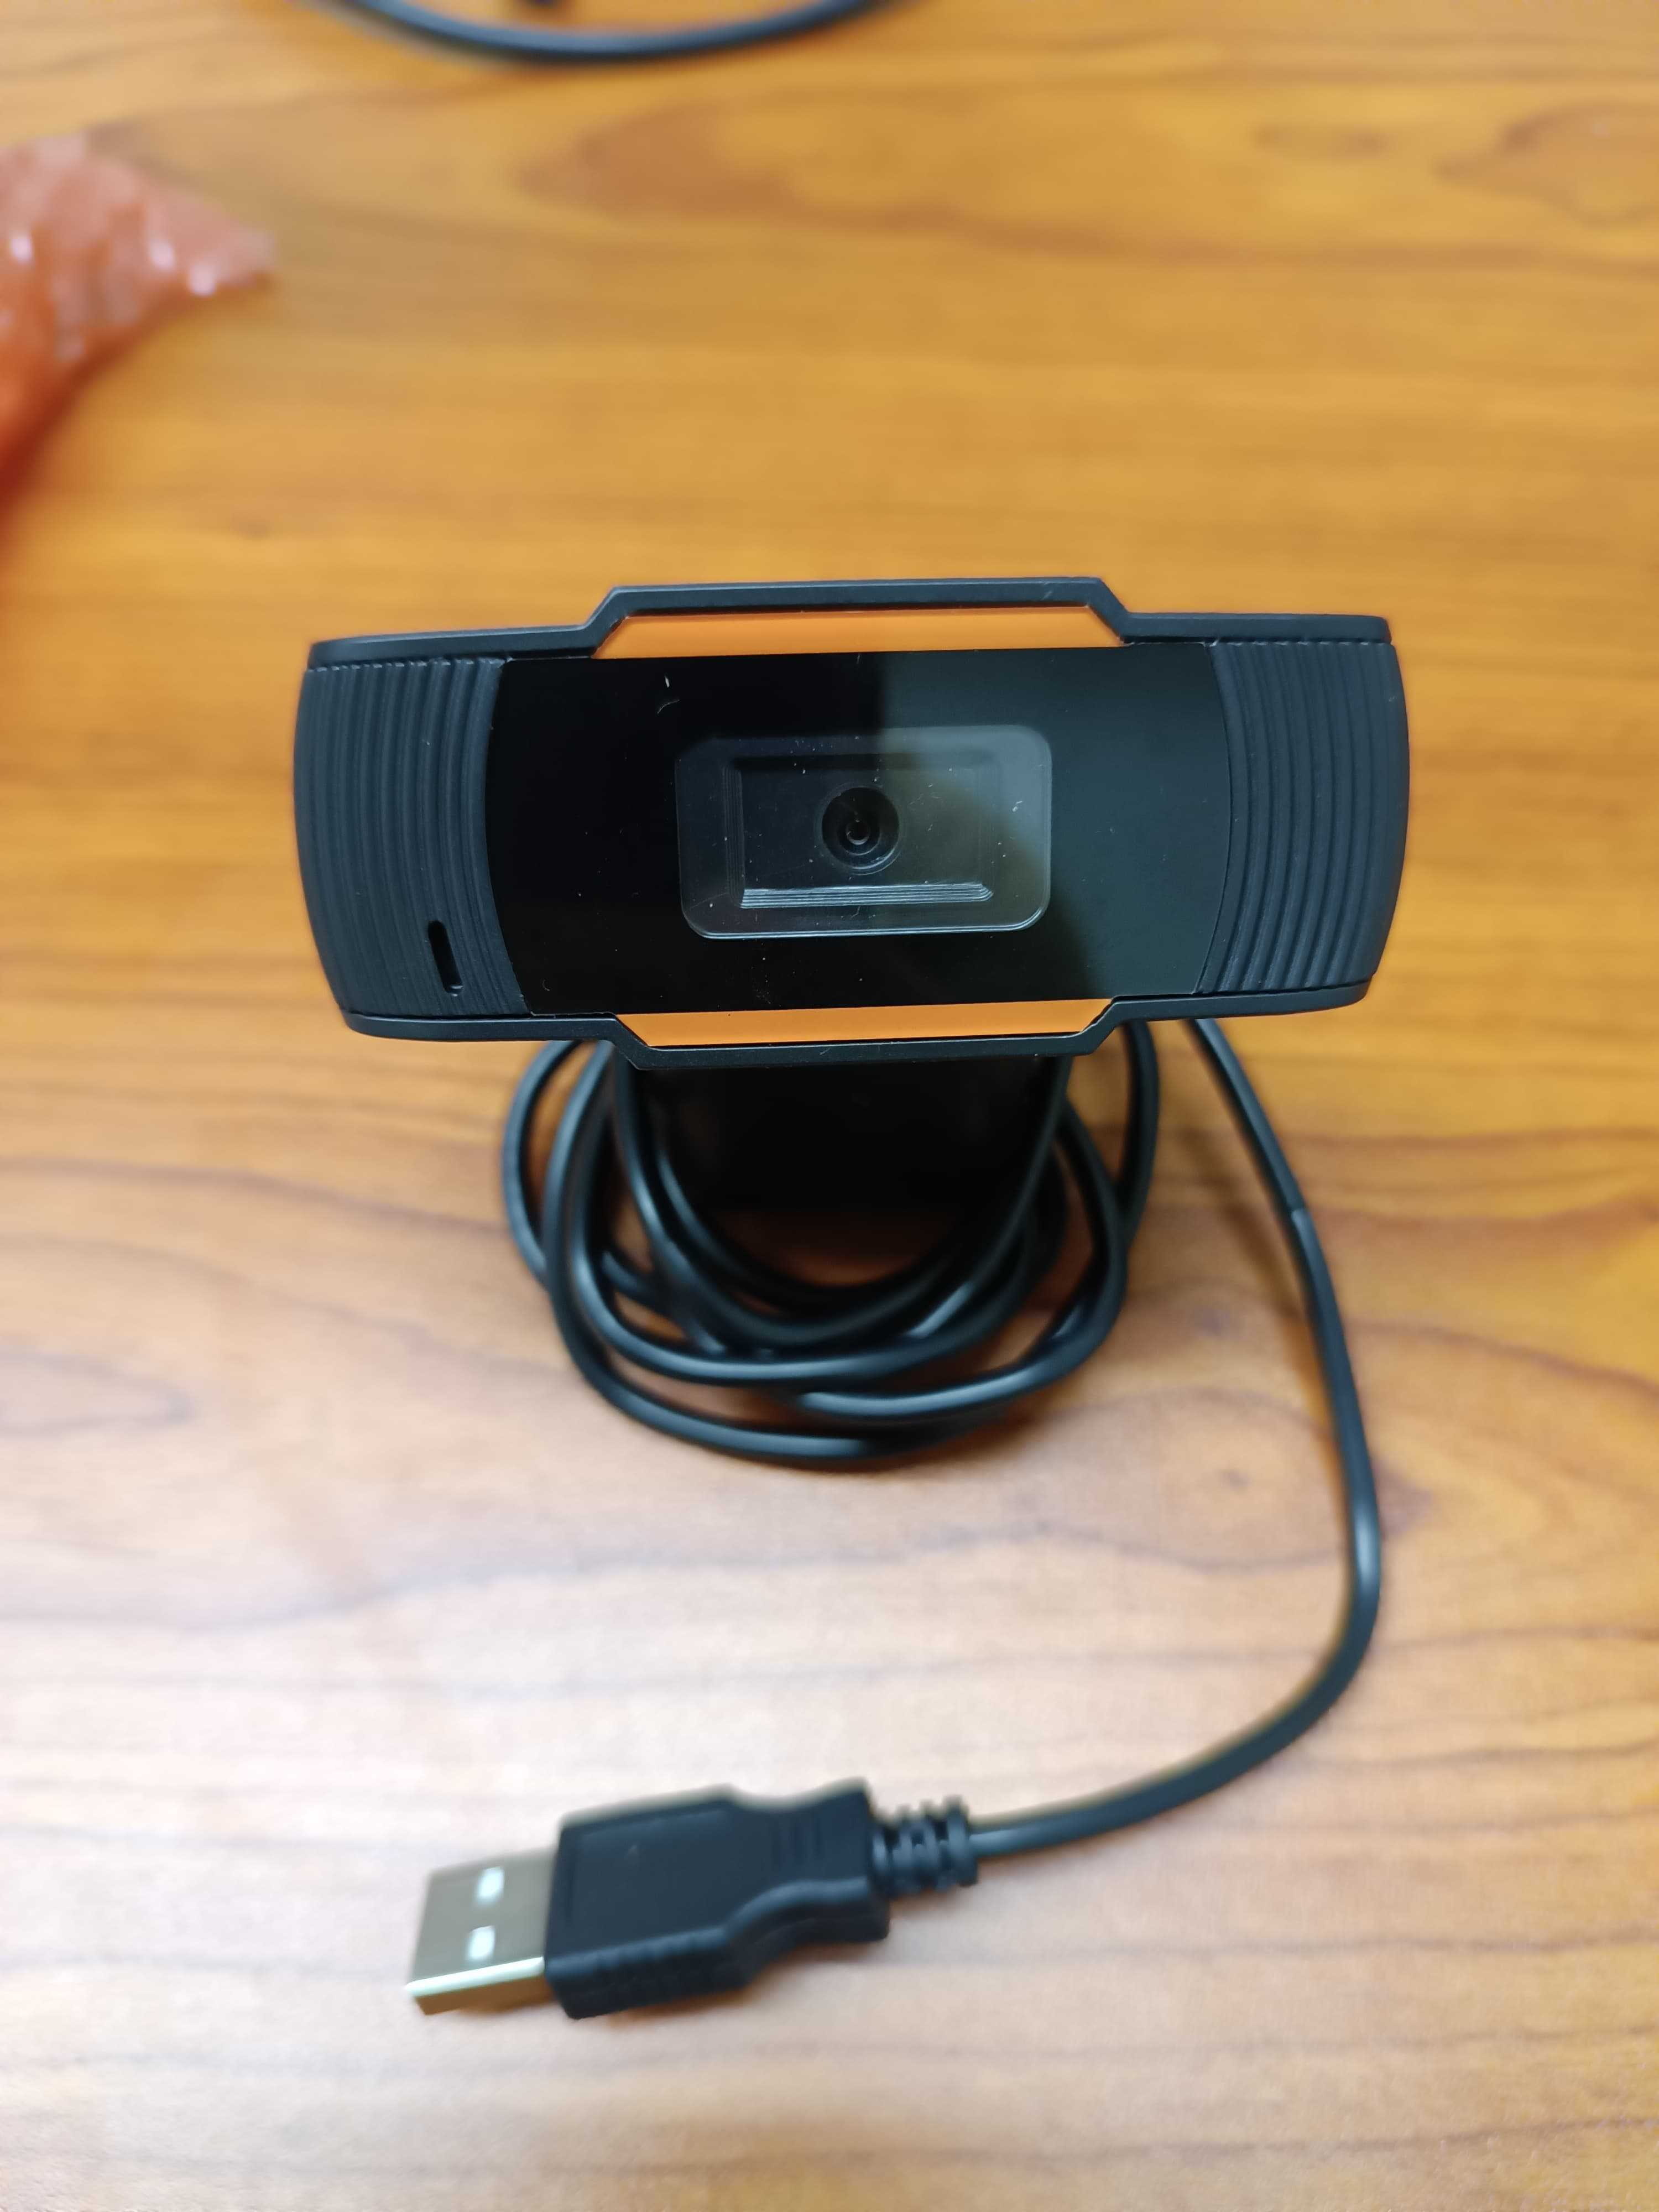
\includegraphics[width=0.3\linewidth]{figures/webcam}
    \caption{Webcam used to capture the video.}
    \label{fig:camera}
\end{figure}

In order to implement the gNB and the UE in two different host computers, we used two Software-Defined Radios (SDRs).
OAI recommends the use of three SDR models: USRP B210, USRP N300, and USRP X300\@ \cite{openairinterface_tutorial}.
For our implementation, we have selected the first model since it is cost-effective and popular within the community.
This model uses a USB 3.0 interface to connect to the computer that acts as a processing unit.
The SDR was equipped with two W5208K dipole antennas.
Figure~\ref{fig:SDRs} shows the two SDRs with their respective antennas.
We selected 3.6 GHz as the carrier frequency for the 5G RAN\@.

\begin{figure}[H]
    \centering
    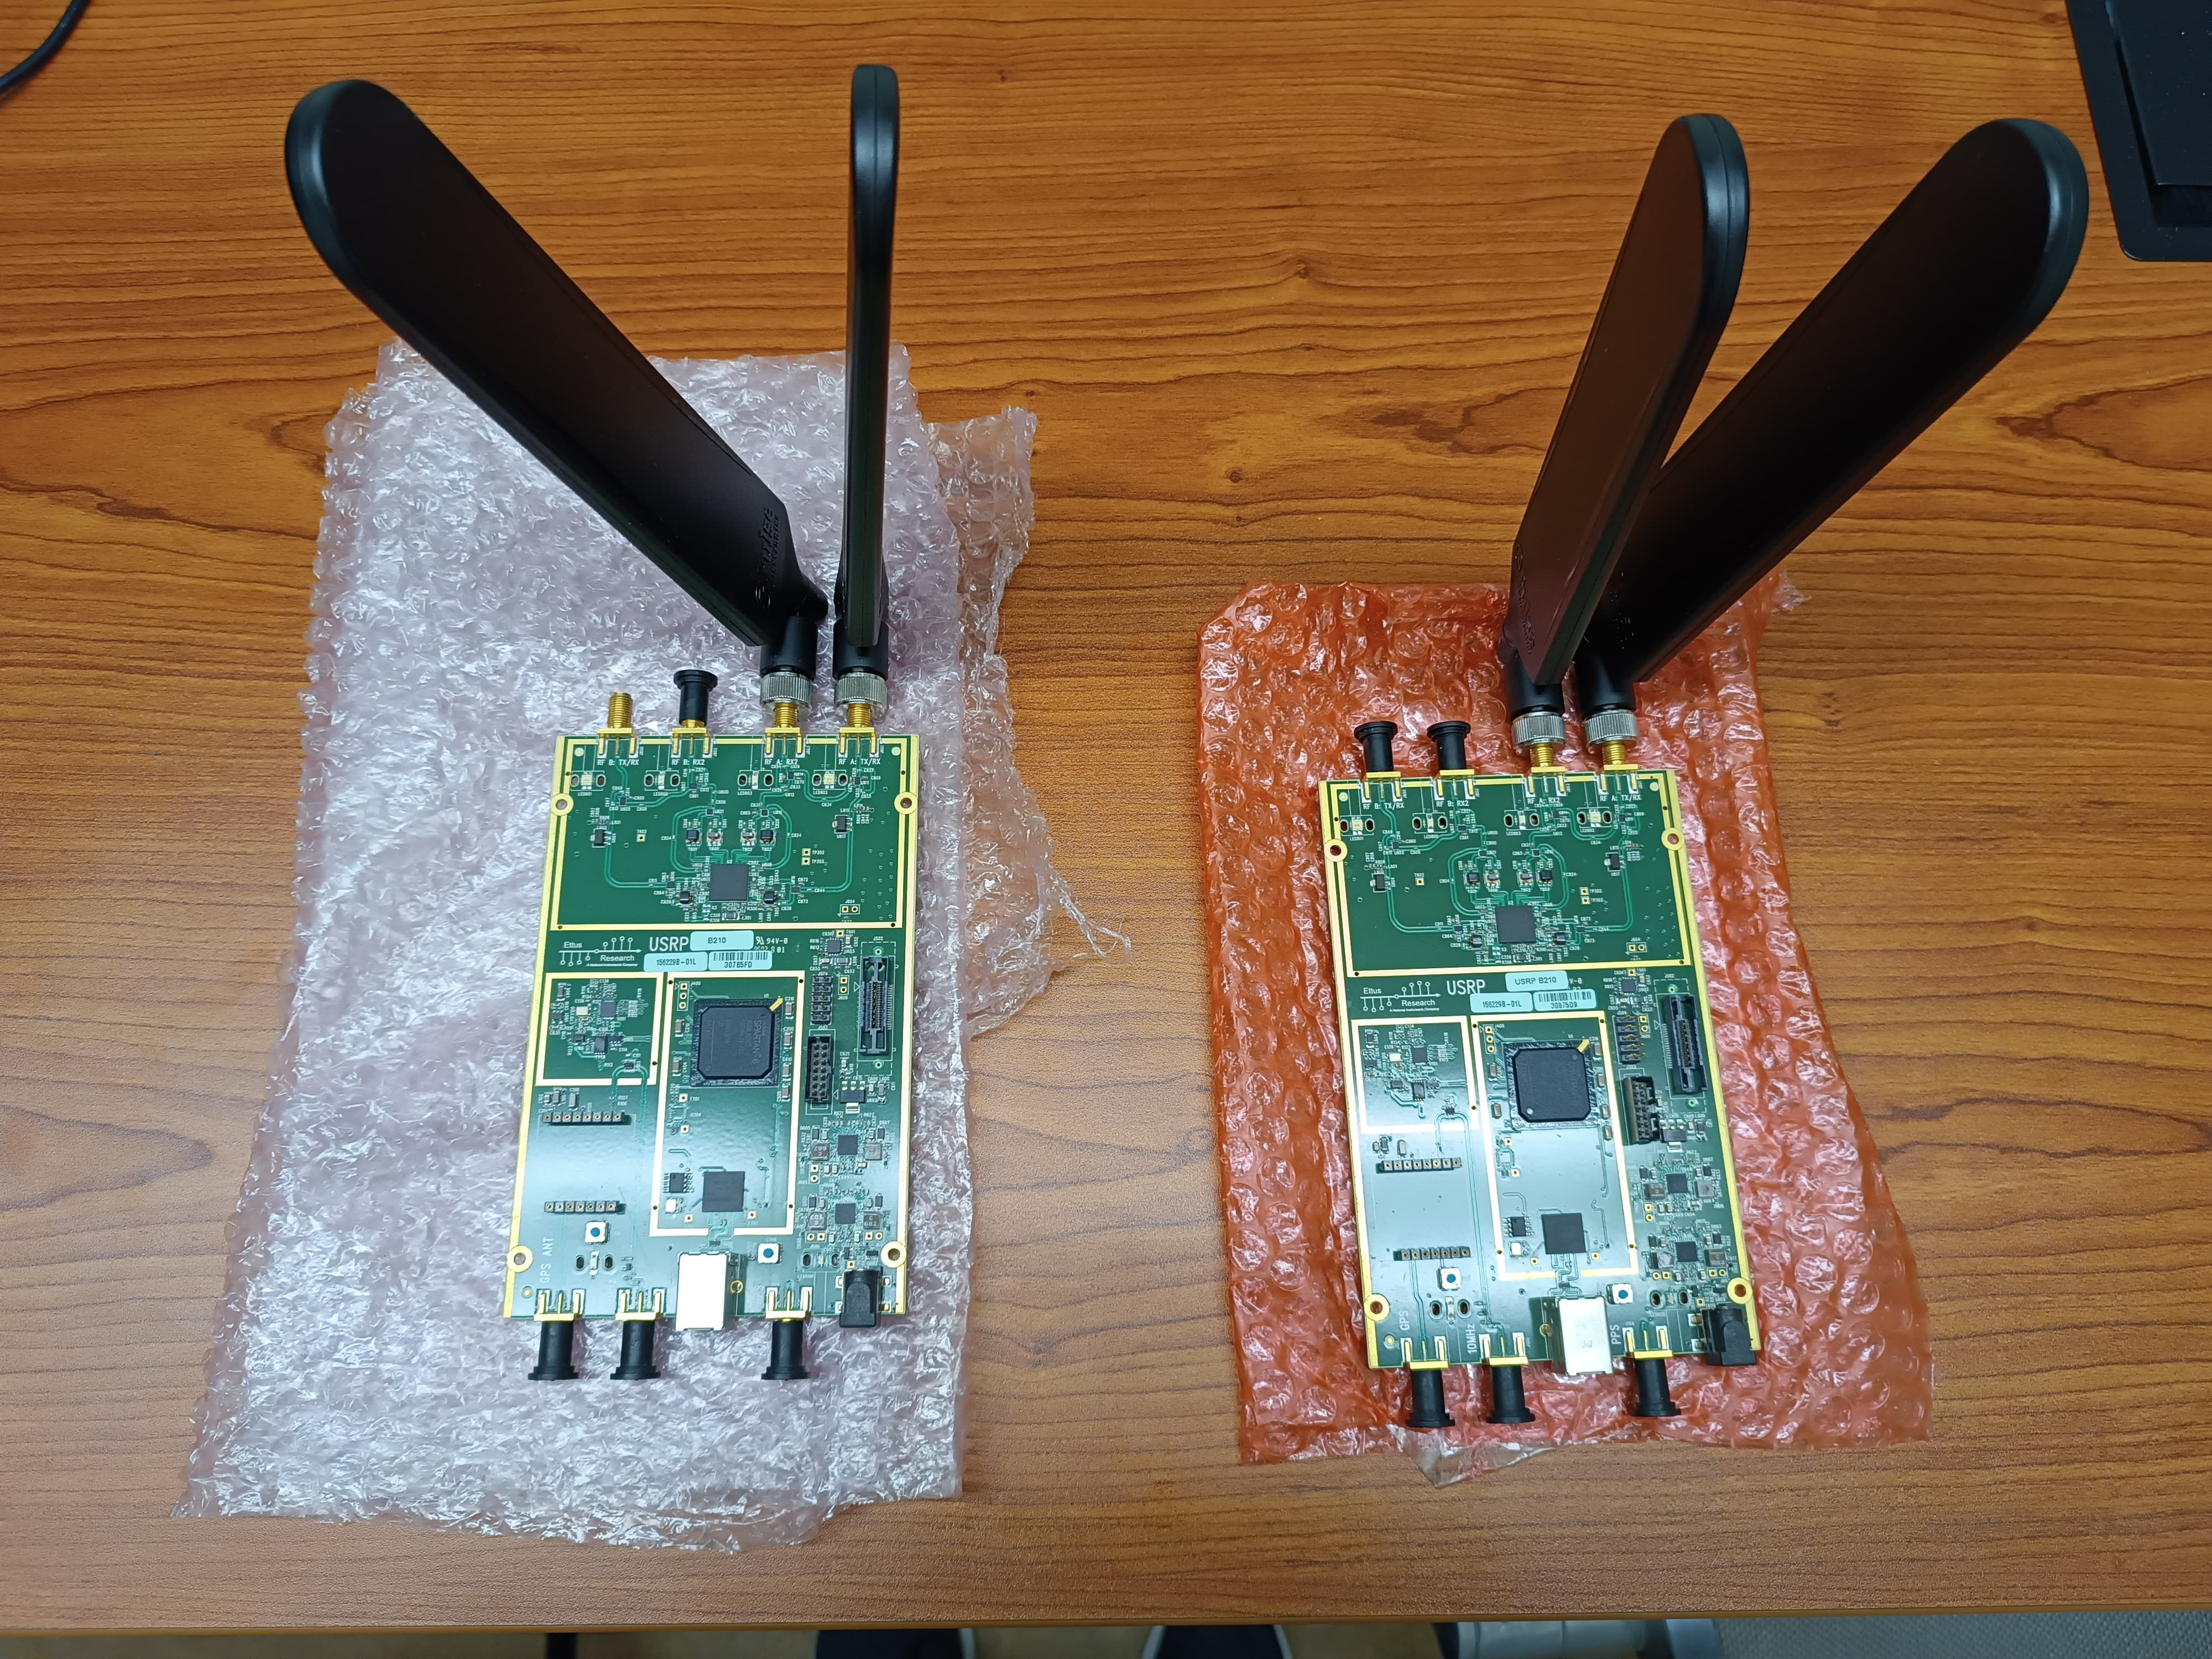
\includegraphics[width=0.5\linewidth]{figures/SDRs}
    \caption{USRP B210 SDRs and their respective antennas.}
    \label{fig:SDRs}
\end{figure}



\subsubsection{UE}
The UE was deployed on an HP EliteBook 840 Laptop, shown in Figure~\ref{fig:computer_hp}.
The hardware requirements for deploying the UE are 8 cores and 8 GB of RAM\@.
Table~\ref{tab:specs_pc_ue} depicts the specifications of the computer responsible for the UE\@, confirming that the hardware is compatible wth the UE software requirements.
The UE used the USRP B210 SDR to communicate with the gNB\@.

\begin{figure}[H]
    \centering
    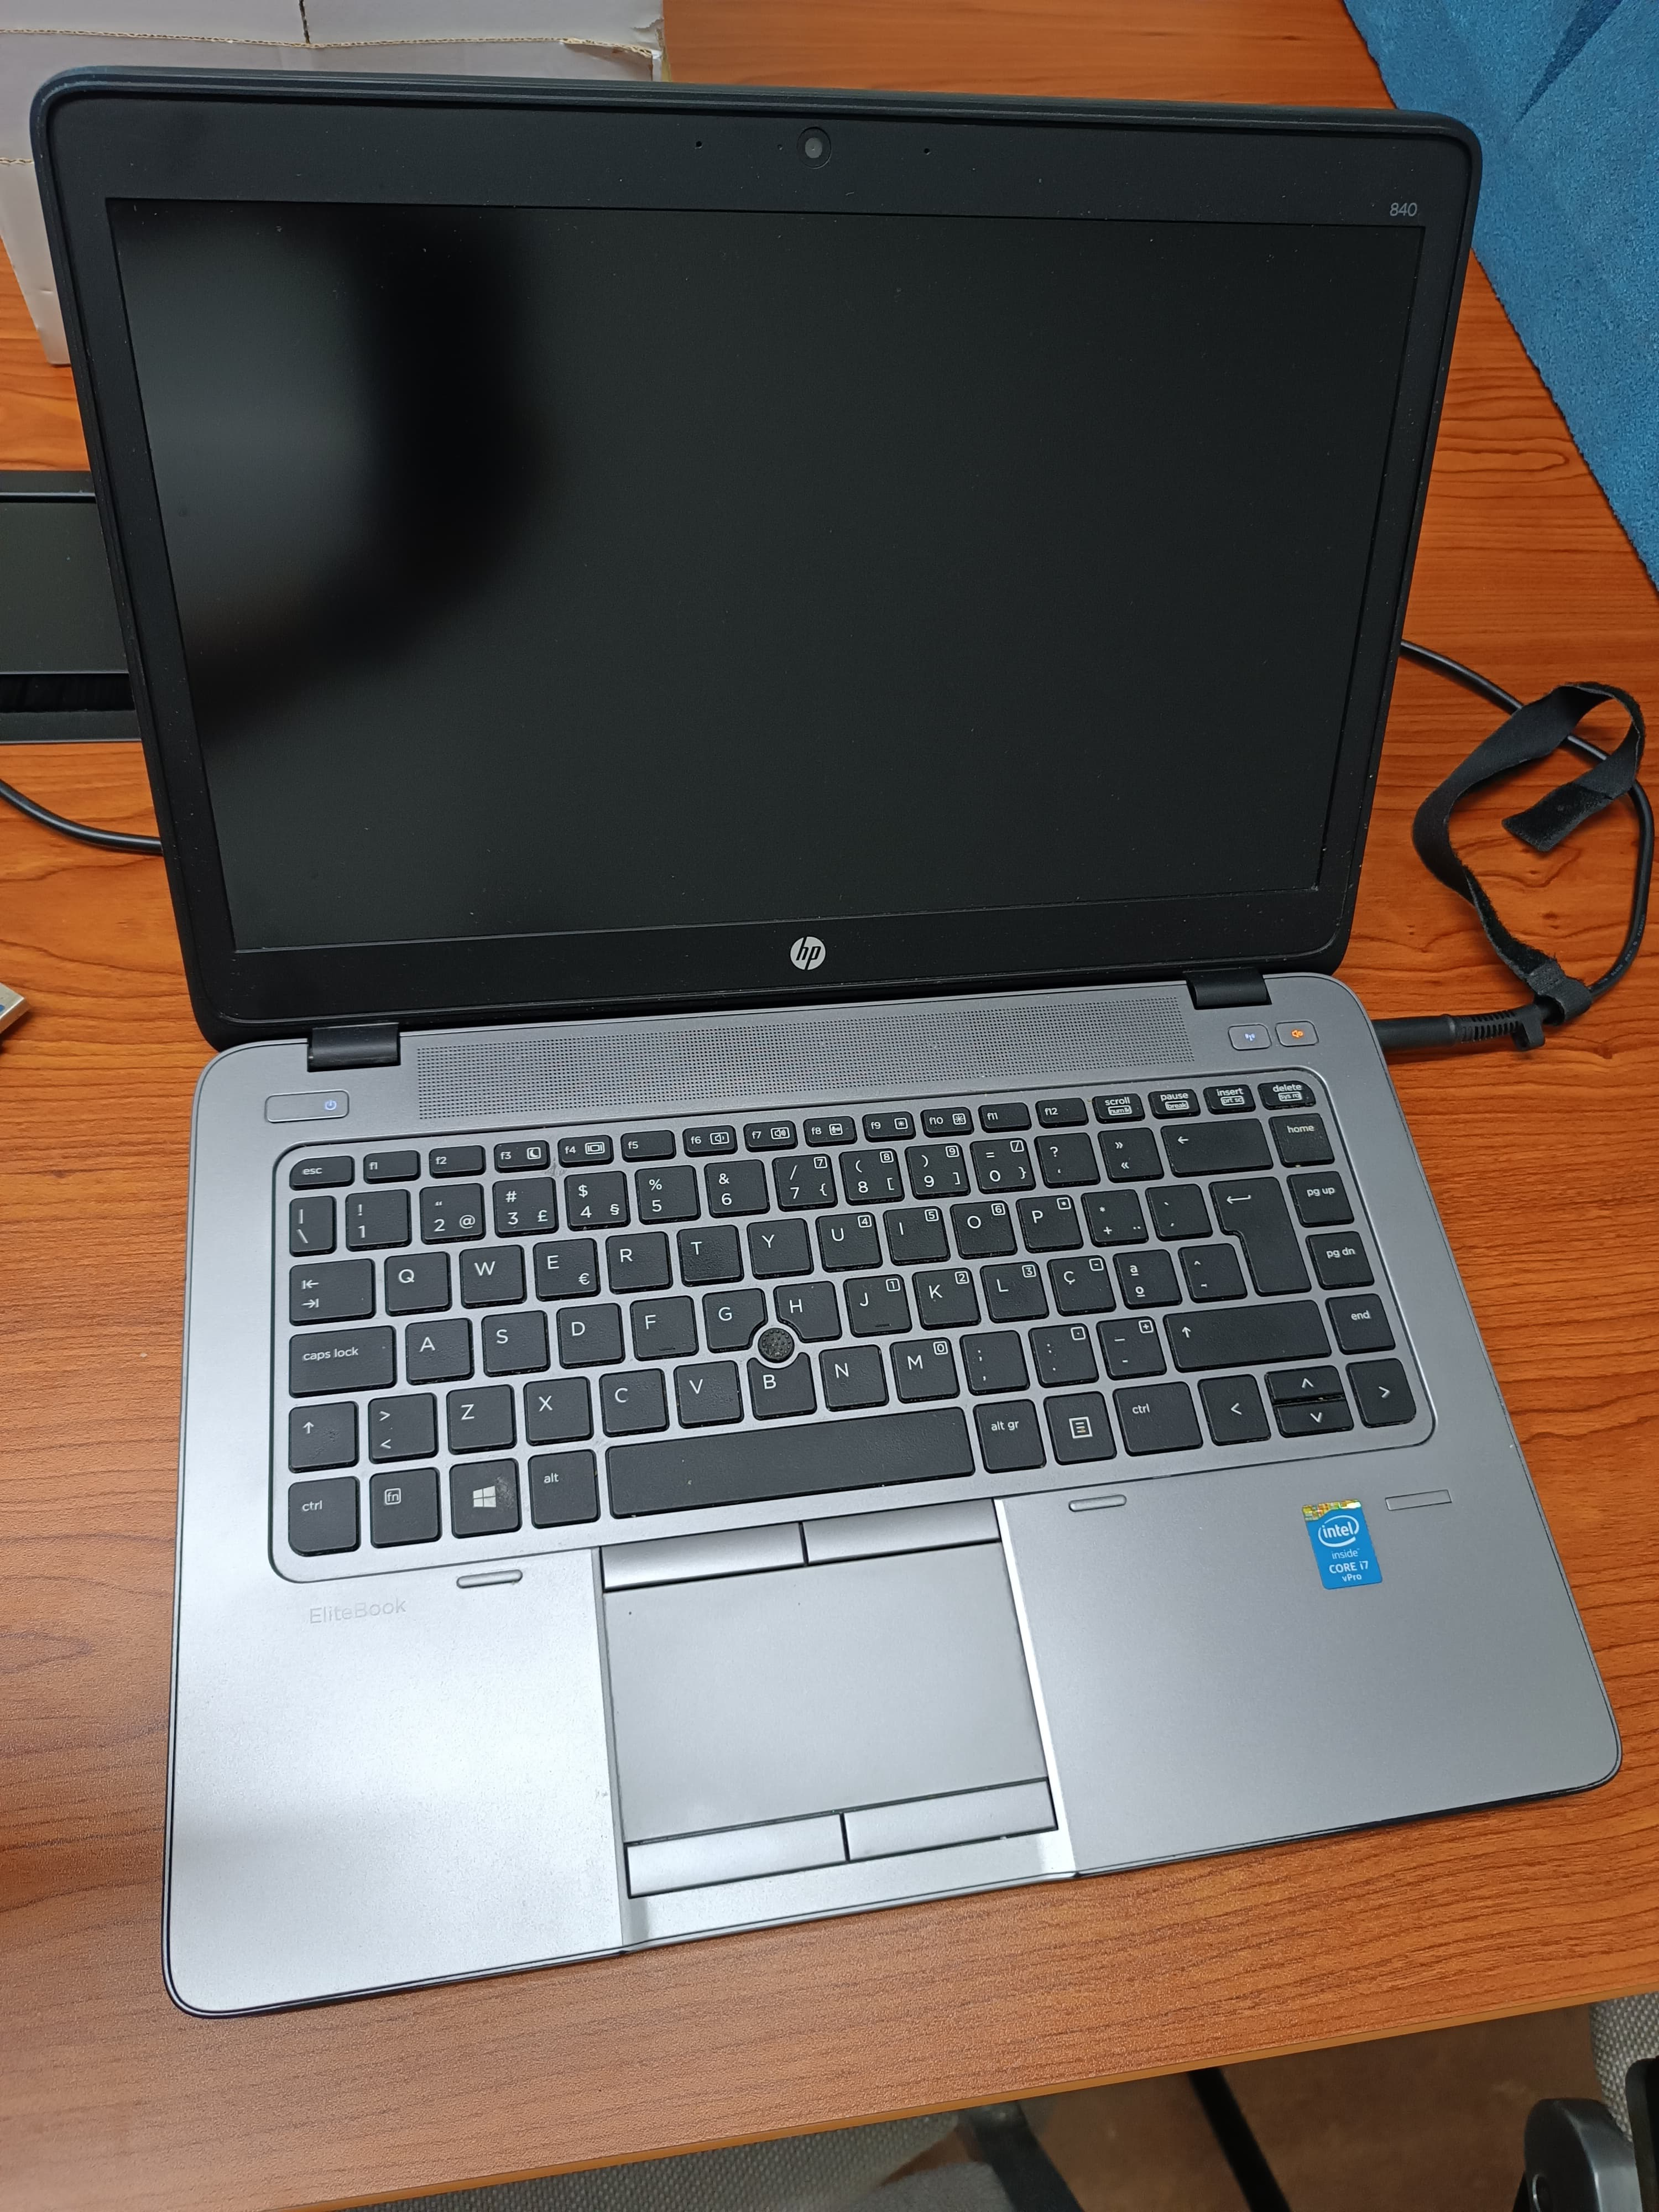
\includegraphics[width=0.3\linewidth]{figures/hp}
    \caption{HP EliteBook 840 Laptop.}
    \label{fig:computer_hp}
\end{figure}

\begin{table}[H]
    \caption{Specifications of the HP EliteBook 840.}
    \label{tab:specs_pc_ue}
    \begin{tabular}{|c|c|}
        \hline
        \textbf{Specification} & \textbf{Details} \\ \hline
        Processor                      &  Intel(R) Core(TM) i7-5600U CPU @ 2.6 GHz          \\ \hline
        RAM                      &          16 GB        \\ \hline
        Disk                      &   128 GB         \\ \hline
        GPU                     &   Intel Corporation HD Graphics 5500                \\ \hline
        Operating System & Ubuntu 22.04.4 LTS                  \\ \hline  %  check
    \end{tabular}
\end{table}


\subsection{Vision Module}\label{subsec:vision-module}
Our vision module is implemented as a Python server, designed to interface with the xApp (its client) via an SCTP socket over the Loopback interface (127.0.0.1) on port 4321.
The module manages the following functions:

\begin{itemize}
\item Information exchange: Facilitates communications between the server and client.
\item Detection and tracking: Identifies and tracks objects within the video feed.
\item Image processing: Processes video data to derive environmental information.
\item Utility operations: Performs various supportive tasks (such as conversion of coordinates and calculation of intersecting bounding boxes) to enhance overall functionality.
\end{itemize}

To ensure timely and efficient video processing, we utilize a multi-threading approach:

\begin{enumerate}
\item Communications thread: Manages the connection with the client, handling message exchanges and maintaining seamless communications.
\item Processing thread: Focuses on video analysis, including object identification, while generating messages based on the environmental data processed from the video stream.
\end{enumerate}

For optimized performance in handling the computationally intensive tasks of image processing, we leverage GPU acceleration.
We selected the nano version, YOLOv8n, due to its reduced parameter count, making it less resource-intensive and better suited to our solution.
This choice significantly accelerates processing times and reduces CPU load, enhancing overall system efficiency and responsiveness.
The combination of GPU utilization and the streamlined YOLOv8n model ensures effective operation of our module.



\subsection{OAI 5G Core Network}\label{subsec:oai-5g-core-network}
OAI offers three methods for implementing the Core Network: bare-metal installation or virtual machines, automated deployment of network functions (NFs) in Docker containers using Docker-Compose, and cloud-native deployment using Helm Chart on OpenShift or Kubernetes clusters ~\cite{oai5gcore}.
Choosing Docker for deployment simplifies the process by encapsulating network functions in containers, making them easier to manage, scale, and automate, while enhancing the overall efficiency and flexibility of the network infrastructure.
Figure~\ref{fig:core_depl} shows a diagram of the deployed 5G Core containers, version v1.5.1~\cite{oai-cn5g-fed-v1.5.1}.
It also presents the configuration commands necessary to properly forward traffic to and from the Core Network containers.
The IP addresses for each Core Network component and Data Network can be seen in Table~\ref{tab:ip_core} and Table~\ref{tab:ip_dn}, respectively.


\begin{figure}[H]
    \centering
    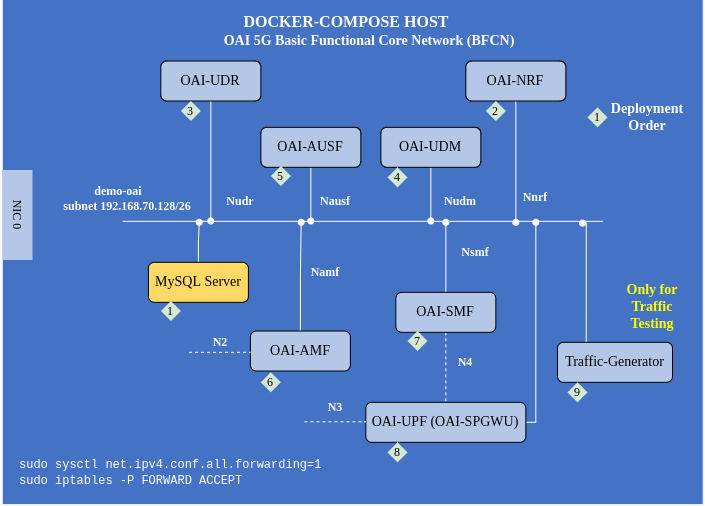
\includegraphics[width=0.7\linewidth]{figures/core_deply}
    \caption{Core deployment diagram~\cite{oai_cn5g_fed_deploy}.}
    \label{fig:core_depl}
\end{figure}


\begin{table}[H]
    \caption{Deployed 5G Core Network functions IP addresses.}
    \label{tab:ip_core}
    \centering
    \resizebox{0.3\textwidth}{!}{%
        \begin{tabular}{|c|c|}
            \hline
            \textbf{Core Network Function} & \textbf{IP} \\ \hline
            NRF & 192.168.70.130 \\ \hline
            MySQL & 192.168.70.131\\ \hline
            AMF & 192.168.70.132 \\ \hline
            SMF & 192.168.70.133 \\ \hline
            UPF & 192.168.70.134 \\ \hline
            UDR & 192.168.70.136 \\ \hline
            UDM & 192.168.70.137 \\ \hline
            AUSF & 192.168.70.138 \\ \hline
        \end{tabular}}
\end{table}

\begin{table}[H]
    \caption{Deployed data network components IP addresses.}
    \label{tab:ip_dn}
    \centering
    \resizebox{0.3\textwidth}{!}{%
        \begin{tabular}{|c|c|}
            \hline
            \textbf{Core Network Function} & \textbf{IP} \\ \hline
            UPF & 192.168.70.134 \\ \hline
            External-DN & 192.168.70.135 \\ \hline
        \end{tabular}}
\end{table}

\subsection{OAI gNB}\label{subsec:oai-gnb}
For the deployment of the OAI gNB, we used the latest version of OAI RAN, following the steps present in~\cite{openairinterface5g_e2ap}.
Besides the steps described in the tutorial, deploying the gNB with the SDR, it was required changing the \textit{gnb.sa.band78
.fr1.106PRB.usrpb210.conf} configuration file.
Specifically, edit Mobile Country Code (MCC), Mobile Network Code (MNC), and Tracking Area Code (TAC) values to ensure they corresponded to the values present in the Core \textit{docker-compose.yaml} file.
Figure~\ref{fig:gnb_conf} depicts the changes, in lines 13 and 14 of the file to comply with the 5G Core Network values.
If these values do not align, the NGAP setup between AMF and gNB over the N2 interface fails.
It was also necessary to modify the IP address of the AMF and assign an IP so that the gNB was able to communicate with the AMF and SMF\@.

\begin{figure}[H]
    \centering
    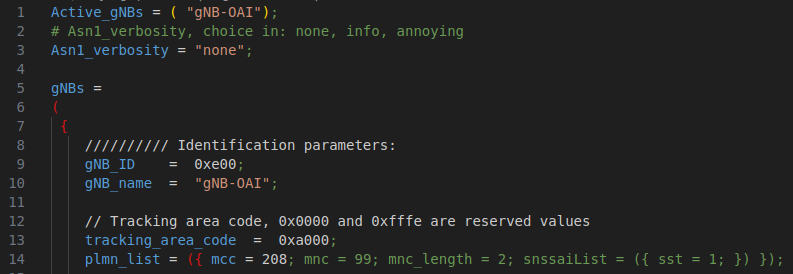
\includegraphics[width=0.7\linewidth]{figures/gnb_conf}
    \caption{Intial segment of textit{gnb.sa.band78
    .fr1.106PRB.usrpb210.conf} configuration file, with the respective MCC, MNC and TAC values}
    \label{fig:gnb_conf}
\end{figure}

Besides configuring the fields above, it was also necessary to configure the proper IP address for the AMF\@.
As presented in Table~\ref{tab:ip_core}, such IP address is 192.168.70.132.
Following that, we set the IP that the gNB uses to communicate with the AMF and SMF\@.
We have chosen to use a Wi-Fi link for this purpose.


Finally, it was necessary to establish a connection between the OAI gNB software and the SDR\@.
As recommended by OAI, we used the USRP Hardware Driver (UHD)~\cite{uhdusrpdriver}.
UHD is a driver that enables communication between software and USRP hardware, providing a standardized interface for configuring and controlling aspects of the SDR devices, such as frequency, sample rate, gain, and antenna settings.
Figure~\ref{fig:uhd_probe} illustrates the UHD driver detecting USRP device, loading its firmware, and performing diagnostic tests.

\begin{figure}[H]
    \centering
    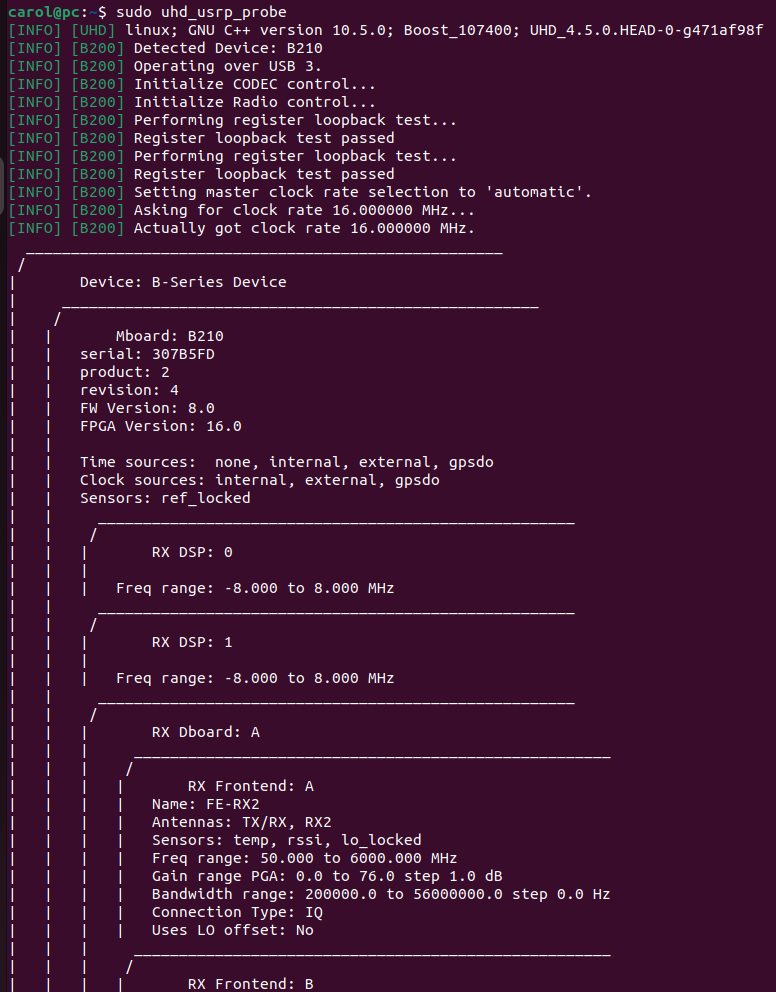
\includegraphics[width=0.5\linewidth]{figures/uhd_usrp_probe}
    \caption{UHD obtaining information about the connected USRP device and testing it}
    \label{fig:uhd_probe}
\end{figure}

\subsection{OAI 5G UE}\label{subsec:oai-5g-ue}
In order to deploy the OAI UE, we needed to initiate the OAI UE software modem with parameters corresponding to the gNB settings.
The command used was:

\lstinline[columns=flexible,breaklines=true]{sudo ./nr-uesoftmodem -r 106 --numerology 1 --band 78 -C 3619200000 --ue-fo-compensation --sa -E --uicc0.imsi 208990200000001}


The parameters include:

\begin{itemize}
    \item \texttt{-r 106}: Sets the channel bandwidth in terms of Resource Blocks (RBs), to 106.
    \item \texttt{--numerology 1}: Specifies the numerology index, set to 1, defining subcarrier spacing and slot duration.
    The gNB must use the same numerology index for compatibility.
    \item \texttt{--band 78}: Configures the UE to operate in the n78 band, with the gNB is also set to operate in the same frequency.
    \item \texttt{-C 3619200000}: Sets the center frequency to 3619.2 MHz, which the gNB is also configured to transmit.
    \item \texttt{--ue-fo-compensation}: Enables frequency offset compensation for the UE, to ensure synchronization with the gNB\@.
    \item \texttt{--sa}: Indicates that the UE is operating in standalone mode, directly connecting to the 5G network without relying on an LTE anchor, thus matching the gNB configuration.
    \item \texttt{-E}: Specifies that the program should utilize 75\% of the sampling frequency.
    \item \texttt{--uicc0.imsi 208990200000001}: Sets the IMSI of the UE to \texttt{208990200000001}.
\end{itemize}

We needed to use one of the International Mobile Subscriber Identity (IMSI) values from the Core database to ensure the UE could authenticate successfully.
The IMSI value \texttt{208990200000001} was selected from the 5G Core database and used in the \texttt{nr-uesoftmodem} command.
This selection was crucial as it aligns with the subscriber information stored in the network, facilitating proper authentication and allowing the UE to connect and communicate with the network.
Ensuring that the IMSI used in the UE configuration matches an entry in the Core database, enables that the UE can authenticate correctly and access the network services.

\subsection{FlexRIC}\label{subsec:flexric}
FlexRIC is deployed on the same computer as the OAI 5G Core Network.
The procedure involves installing the required dependencies and compiling FlexRIC software.
By default, FlexRIC is configured to run on the Loopback Interface address (127.0.0.1).
Since we are deploying gNB and FlexRIC on the same host, this did not need to be to changed.
In order to ensure the use of the E2 Agent, it was necessary to include the following information in the configuration file:

\begin{verbatim}
e2_agent = {
  near_ric_ip_addr = "127.0.0.1";
  sm_dir = "/usr/local/lib/flexric/"
}
\end{verbatim}

This indicates that FlexRIC is running on the localhost IP, while the RIC is running on the same machine as the E2 agent.
The directory specifies where the Service Models for FlexRIC are located.
This is essential to ensure the correct communications between OAI gNB and FlexRIC\@.

\subsection{xApp}\label{subsec:xapp}
To enhance the functionality and adaptability of our 5G network, we developed an xApp designed to receive and process messages from the Vision Module.
The xApp operates by combining the decoded location data with Signal-to-Noise Ratio (SNR) values from the network.
By analyzing this information, the xApp makes automated decisions regarding the optimal positioning of the gNB\@.
Specifically, if the SNR values indicate that the gNB's current location is not adequate due to obstacles, the xApp prints a message indicating the need to move the gNB\@.
This dynamic adjustment aims at maintaining optimal SNR, ensuring better network performance and reliability.

\textcolor{red}{EXPAND WITH THE maquina de estados}

\section{Summary}\label{sec:summary}
The proposed architecture consits of two logical units.
The first unit comprises the OAI 5G Core Network, FlexRIC, xApp, and Vision Module, deployed on an Acer Aspire laptop.
The second unit includes the OAI UE, deployed on an HP Elitebook laptop.
The gNB and the UE use USRP B210 SDR to connect via 5G wireless link.
The Vision Module receives a video feed, processes it, and sends relevant obstacle information from the video via its interface.
The xApp is responsible for monitoring the received messages and the SNR between gNB and UE\@.
In summary, this chapter details how we integrated CV in 5G OAI as a novel solution for improved RAN\@.






